\documentclass[varwidth]{standalone}
\usepackage{subcaption}
\usepackage{caption}
\usepackage{graphicx}

\captionsetup[subfigure]{
justification=centering, % <<< label and text on different lines
  singlelinecheck=true}

\begin{document}

 
\begin{figure}
  \begin{subfigure}[b]{6cm}
    \centering
    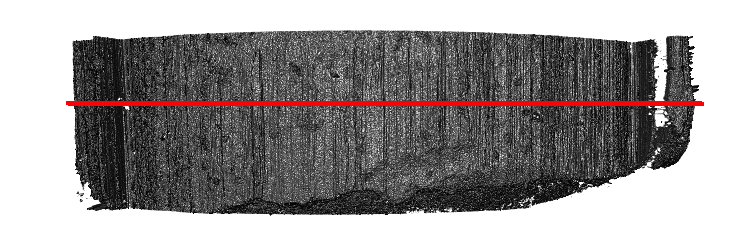
\includegraphics[width=0.8\textwidth]{../images/3d_plot_top_crosscut}
        \captionsetup{justification=centering}
    \caption*{Step 1: 3D scan with identified horizontal crosscut}

  \end{subfigure}
  \hfill
  \begin{subfigure}[b]{6cm}
    \centering
    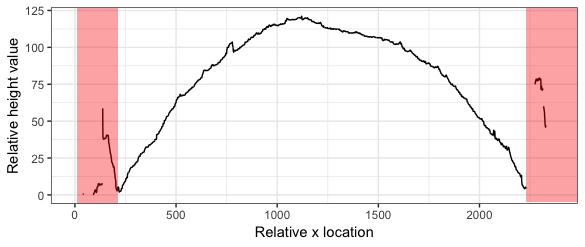
\includegraphics[width=0.8\textwidth]{../images/profile_paper}
            \captionsetup{justification=centering}
    \caption*{Step 2: Horizontal crosscut with identified GEA data}
  \end{subfigure} \\
  
  \begin{subfigure}[b]{6cm}
    \centering
    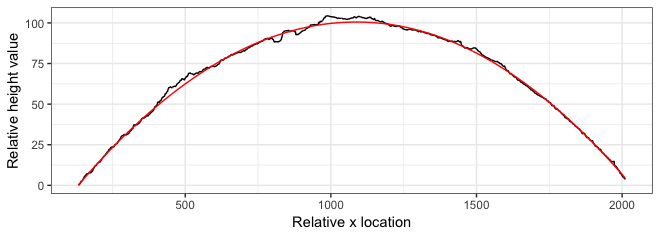
\includegraphics[width=0.8\textwidth]{../images/profile_paper_loess}
            \captionsetup{justification=centering}
    \caption*{Step 3: Non-parametric curvature estimation}
  \end{subfigure}
 \hfill
  \begin{subfigure}[b]{6cm}
    \centering
    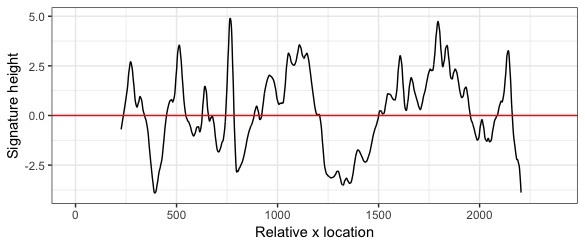
\includegraphics[width=0.8\textwidth]{../images/signature_paper}
            \captionsetup{justification=centering}
    \caption*{Step 4: Extracted LEA  \\  signature}
  \end{subfigure}
\end{figure}
 
\end{document}
